\documentclass[tikz,border=4pt]{standalone}
\usepackage{ctex}
\usepackage{amsmath}
\usepackage{pgfplots}
\pgfplotsset{compat=1.18}
\usetikzlibrary{calc, arrows.meta}

\begin{document}
% part14/04 动点最值示意图
% 抛物线 y=x^2-2x, P在[0,3]上的动点, 直线y=x, 求最大距离
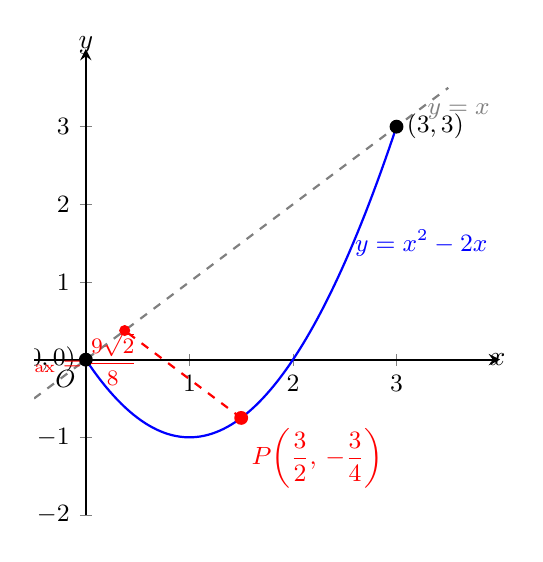
\begin{tikzpicture}
\begin{axis}[
  axis lines=center,
  xlabel={$x$}, ylabel={$y$},
  every axis x label/.style={at={(axis cs:3.8,0)}, anchor=west},
  every axis y label/.style={at={(axis cs:0,3.8)}, anchor=south},
  xmin=-0.5, xmax=4, ymin=-2, ymax=4,
  xtick={0,1,2,3},
  ytick={-2,-1,0,1,2,3},
  tick label style={font=\small},
  width=7.5cm, height=7.5cm,
  thick,
]
  % 抛物线 y=x^2-2x (0<=x<=3)
  \addplot[blue, thick, domain=0:3, samples=80] {x^2-2*x};
  \node[blue, right, font=\small] at (axis cs:2.5,1.5) {$y=x^2-2x$};

  % 直线 y=x
  \addplot[gray, thick, dashed, domain=-0.5:3.5] {x};
  \node[gray, right, font=\small] at (axis cs:3.2,3.2) {$y=x$};

  % 端点
  \fill (axis cs:0,0) circle(2.5pt);
  \node[left, font=\small] at (axis cs:0,0) {$(0,0)$};
  \fill (axis cs:3,3) circle(2.5pt);
  \node[right, font=\small] at (axis cs:3,3) {$(3,3)$};

  % 最值点P(3/2, -3/4)
  \fill[red] (axis cs:1.5,-0.75) circle(2.5pt);
  \node[below right, red, font=\small] at (axis cs:1.5,-0.75) {$P\!\left(\dfrac{3}{2},\,-\dfrac{3}{4}\right)$};

  % P到直线的垂线（y=x即x-y=0，垂线方向为(1,1)/sqrt(2)）
  % 垂足Q：P + t(1,1) 使其在y=x上，t=((1.5+0.75)/2)=1.125/2=...
  % Q的坐标：Q=(1.5+0.375, -0.75+0.375)=(1.875, 0.375)...
  % 简化：Q在y=x上最近点：Q=((1.5-0.75)/2+{(1.5+0.75)/2},{same})
  % Q = ((xP+yP)/2, (xP+yP)/2)=(0.375, 0.375)
  \fill[red] (axis cs:0.375,0.375) circle(2pt);
  \draw[red, dashed] (axis cs:1.5,-0.75) -- (axis cs:0.375,0.375);
  \node[red, font=\footnotesize, left] at (axis cs:0.6,0.0) {$d_{\max}=\dfrac{9\sqrt{2}}{8}$};

  \node[below left, font=\small] at (axis cs:0,0) {$O$};
\end{axis}
\end{tikzpicture}
\end{document}
